%% template.tex - Template for a snapshot of modern mathematics from Oberwolfach.
%
% The following authors contributed to the initial version of this work (in alphabetical order):
%   Carla Cederbaum (concept, testing)
%   Konrad Renner (design)
%   Christian Stussak (programming)
%
% with additional support by
%   Sophia Jahns (testing)
%   Christoph Knoth (design)
%   Andreas Daniel Matt (concept)
%   Lea Renner (testing)
%
% To the extent possible under law, the author(s) have dedicated all copyright
% and related and neighboring rights to this software to the public domain worldwide.
% This software is distributed without any warranty. 
%
% You should have received a copy of the CC0 Public Domain Dedication along with
% this file. If not, see <https://creativecommons.org/publicdomain/zero/1.0/>. 
%
%%

%%% Please use pdflatex for compiling this file.
\documentclass{snapshotmfo}

%%%%%%%%%%%%%%%% WILL BE FILLED OUT BY THE EDITORS ACCORDING TO YOUR SPECIFICATIONS %%%%%%%%%%%%%%%%%%%%%%
%\categorizationmath{algebra and number theory,analysis,discrete mathematics and foundations,geometry and topology,numerics and scientific computing,probability theory and statistics} %at least one must be chosen
%\categorizationconnect{chemistry and earth science,computer science,engineering and technology,finance,humanities and social sciences,life science,physics,reflections on mathematics} %can be void
%\license{CC-BY-SA-4.0} %recommended
%\license{CC-BY-ND-4.0}
%\license{CC-BY-NC-SA-4.0} 
%\snapshotid{id}{year}
%\translator{german}{Trans Lator}
\junioreditor[gs]{will be filled out by the editors}{junior-editors@mfo.de}
% The optional argument of \junioreditor indicates gender (f = female, m = male, g = gender-neutral = default)
% and number (s = singular = default, p = plural).
% The implicit plural indicators ', ' and - depending on the language - ' and ', ' und ', ' y ' are
% deprecated and may not be recognized any more in future versions of snapshotmfo.cls.
% Use the optional argument of \senioreditor and of \director to indicate the gender.
\senioreditor[f]{Carla Cederbaum}{senior-editor@mfo.de}
\director[m]{Gerhard Huisken}

%%% Commands for editing
% Uncomment for collaborative editing:
%\usepackage{trackchanges}
%\addeditor{Johannes}
% Uncomment for proofreading:
%\overfullrule=5pt
%%%%%%%%%%%%%%%%%%%%%%%%%%%%%%%%%%%%%%%%%%%%%%%%%%%%%%%%%%%%%%%%%%%%%%%%%%%%%%%%%%%%%%%%%%%%%%%%%%%%%%%%%%


%%%%%%%%%%%%%%%% PLEASE FILL OUT THE FOLLOWING ITEMS %%%%%%%%%%%%%%%%%%%%%%%%%%%%%%%%%%%%%%%%%%%%%%%%%%%%%

%%% Optional recommended packages
%%% Encoding
\usepackage[utf8]{inputenc}
%%% AMS mathematical facilities:
\usepackage{amsmath,amssymb}
%\usepackage{mathtools}
%%% Consistent quotation marks and citations:
%\usepackage{csquotes}
%%% Enhanced typesetting of units:
%\usepackage{siunitx}  
%\sisetup{per-mode=fraction,fraction-function=\nicefrac}
%%% Wrap text around tables and figures:
%\usepackage{wrapfig}

% Please feel free to use your own macros but please do not change the layout of the snapshot.

% By now the documentclass supports the languages 'USenglish', 'ngerman' and 'spanish'.
% Please submit original snapshots in English or German. The support of Spanish is meant for translations.
% If you change the language setting, please delete the .aux file in advance or run your LaTeX compiler *twice*.
%\usepackage[USenglish]{babel}
%\usepackage[ngerman]{babel}
\usepackage[spanish]{babel}

% an improvement to \dots to be loaded after babel
\usepackage{ellipsis}

%%% Please separate your names by \and if there are several authors.
\author{Author One\thanks{Author One is supported by the Mathematical Dreams Come True Foundation.} \and Author Two}

%%% Please insert the title of your snapshot.
\title{Your title}
%%% The content of \title, \begin{abstract}...\end{abstract}, \section, and \subsection will be used for pdf bookmarks
% or pdf metadata or both. Math mode, TeX control sequences, and some special characters will result in hyperref warnings
% like "Token not allowed in a PDF string" and - more seriously - corrupt text in the bookmarks and metadata, resp..
% In case of \title, please use the following variant, if necessary: 
%\title{\texorpdfstring{Your title}{This is a plain text equivalent of your title used for the pdf bookmark and the pdf metadata.}}
% The other control sequences offer a more elegant way to supply the alternative text, see below.

%%% Please provide some information on the author(s).
\authorinfo{\authorname{Author One} is a professor of pure mathematics at the First University.}
\authorinfo{\authorname{Author Two} is a lecturer in applied mathematics at the Second Institution.}

%%%%%%%%%%%%%%%% BIBLIOGRAPHY %%%%%%%%%%%%%%%%%%%%%%%%%%%%%%%%%%%%%%%%%%%%%%%%%%%%%%%%%%%%%%%%%%%%%%%%%%%%
%%% There are three ways to provide your references:
%%% 
%%% 1. by using the embedded .bib file:
%%%    * replace the references below by your own ones
%%%    * and leave the \bibliography command at the end of this file unchanged.
%%% This is the default way as it is a full-fledged BibTex solution
%%% while you have to edit only one file.
%%% 
%%% 2. by using a separate .bib file:
%%%    * provide your own .bib file,
%%%    * delete everything from \begin{filecontents} until \end{filecontents}
%%%    * and make the \bibliography command at the end of this file point to your .bib file.
%%% 
%%% 3. by using no BibTeX at all:
%%%    * delete everything from \begin{filecontents} until \end{filecontents}
%%%    * replace the \bibliography command at the end of this file with the
%%%      thebibliography environment containing a \bibitem command for each reference.
%%% This way is deprecated as it is less flexible than the BibTeX solutions.
%%%
\begin{filecontents}[overwrite]{\jobname.bib}
@book{knuth1984texbook,
  title = {The TeXbook},
  author = {Knuth, D. E.},
  year = {1984},
  edition={1},
  publisher = {Addison-Wesley}
}

@misc{wikiMath,
  author = {Wikipedia},
  title = {Mathematics --- {W}ikipedia{,} The Free Encyclopedia},
  year = {2014},
  url = {https://en.wikipedia.org/wiki/Mathematics},
  urldate = {2014-05-19}
}

@misc{sample13,
  author = {Sample, J.},
  howpublished = {\href{https://arxiv.org/abs/8765.4321v1}{arxiv:8765.4321v1}},
  title = {Interesting facts in mathematics},
  year = {2013}
}

@incollection{sample12,
  author = {Sample, J.},
  title = {Things you don't know about mathematics},
  booktitle = {A bookseries about mathematics},
  publisher = {Some publisher},
  year = {2012}
}

@inproceedings{sample11,
  author={Example, C.},
  title={A new perspective on mathematics},
  booktitle={New perspectives on arts and sciences},
  year={2011}
}

@phdthesis{sample14,
  author={Candidate, A.},
  title={Thesis title},
  school={MFO},
  year={2014}
}
\end{filecontents}
%%%%%%%%%%%%%%%%%%%%%%%%%%%%%%%%%%%%%%%%%%%%%%%%%%%%%%%%%%%%%%%%%%%%%%%%%%%%%%%%%%%%%%%%%%%%%%%%%%%%%%%%%%


%%%%%%%% If your latex file does not compile, please delete all .aux and .log files and try again. %%%%%%%
\begin{document}
%%% Starting with version 1.29 the LaTeX package "bookmark" doesn't create the title bookmark any more.
% As a workaround, please uncomment and edit the following line:
%\pdfbookmark{Your title (without math mode, control sequences and special characters)}{snapshottitle}
% The second argument "snapshottitle" is just an identifier and can be left unchanged.

%%% Please insert your abstract here. 
\begin{abstract}
This is your abstract. It should give a brief overview of your snapshot. If possible, please do not use formulas in your abstract. Please do not use more than 500 characters. 
\end{abstract}
%%% If necessary, use the optional argument to supply an alternative text for the pdf metadata, cf. the comment on \title above: 
%\begin{abstract}[This is a plain text equivalent of your abstract used for the pdf metadata. It should give a brief overview of your snapshot. Please do not use more than 500 characters.]
%This is your abstract containing math mode, TeX control sequences, or some special characters. It should give a brief overview of your snapshot. Please do not use more than 500 characters.
%\end{abstract}

\section{Comment on this unit test: test-template.tex}
test-template.tex differs from template.tex only by this section!
After the following compilations
\begin{verbatim}
pdflatex test-template.tex
bibtex test-template.aux
pdflatex test-template.tex
pdflatex test-template.tex
\end{verbatim}
the following warnings will remain:
\begin{verbatim}
LaTeX Warning: Writing or overwriting file `./test-template.bib'.
Class snapshotmfo Warning: No snapshot id given.
Package isodate Warning: Language spanish unknown to isodate.
Package isodate Warning: Language spanish unknown to isodate.
Class snapshotmfo Warning: No mathematical subject given.
Class snapshotmfo Warning: No connection to other fields given.
Class snapshotmfo Warning: No license information given.
Class snapshotmfo Warning: Unable to compute DOI.

Warning--empty language in sample14
Warning--empty language in sample11
Warning--empty language in knuth1984texbook
Warning--empty language in sample12
Warning--empty language in sample13
Warning--empty language in wikiMath
\end{verbatim}

Using TeXnicCenter with MikTeX on Windows the final compilation summary will read:
\begin{verbatim}
LaTeX-Result: 0 Error(s), 8 Warning(s), 1 Bad Box(es), 5 Pages(s)
BibTeX-Result: 0 Error(s), 6 Warning(s)
\end{verbatim}

The ``overwriting file'' warning is inevitable as long as you provide the references the default
way, i.\,e. as an embedded .bib file.

The ``isodate'' warnings may be ignored as isodate works fine with spanish nonetheless.

The ``class snapshotmfo'' warnings will disappear as soon as you supply the expected information.

Do not make the ``empty language'' warnings disappear by supplying languages for the items,
unless you want the languages explicitely printed in the references!

There may be two extra ``class snapshotmfo'' warnings, which may be ignored, if your hyperref 
package's date is 2020-10-19 or newer.

%%% Please insert the main body of your snapshot here.
\section[Optional plain text substitute for PDF bookmark]{A heading}
Your actual snapshot.\footnote{This is a footnote.} As usual, you can give references such as \cite{knuth1984texbook, wikiMath, sample13, sample12, sample11, sample14} via the \verb+\cite+ command.

We appreciate if you include images or other graphics that illustrate your snapshot. However, please do keep in mind the copyright issues explained in our email in case you include images and graphics you have not produced yourself.

%%% Please use this format to include images. Supported image formats: jpg, pdf, png. Please convert your images to those formats.
\begin{figure}[ht]
        \centering 
        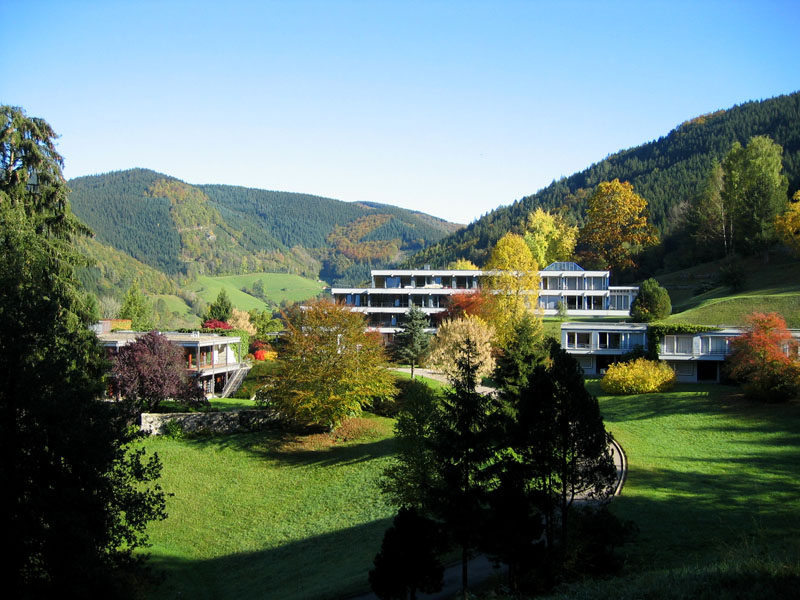
\includegraphics[width= 0.33 \textwidth]{mfo.jpg}
        \caption{An image scaled to 33\% of the textwidth.}
\label{fig:sample-image}
\end{figure}

\subsection{A subsection}
%%% If necessary, use the optional argument to supply an alternative text for the pdf bookmark, cf. the comment on \title above: 
%\subsection[Optional plain text substitute]{A heading containing math mode, for example}
More text and some formulas:
\begin{align}\label{real}
1+1&=2,\\\label{char.2}
1+1&=0.
\end{align}
Formula \eqref{real} refers to $\mathbb{R}$, Formula \eqref{char.2} does not.

\section{More information}
We have composed guidelines to help you write a beautiful and accessible snapshot which you can download at \href{https://www.mfo.de/snapshots/guidelines-for-snapshots}{www.mfo.de/snapshots/guidelines-for-snapshots}. For more information on the snapshot project (including example snapshots), please see \href{https://www.mfo.de/snapshots}{www.mfo.de/snapshots}.

%%% Please use this format to include images. Supported image formats: jpg, pdf, png. Please convert your images to those formats.
\begin{figure}[ht]
        \centering 
        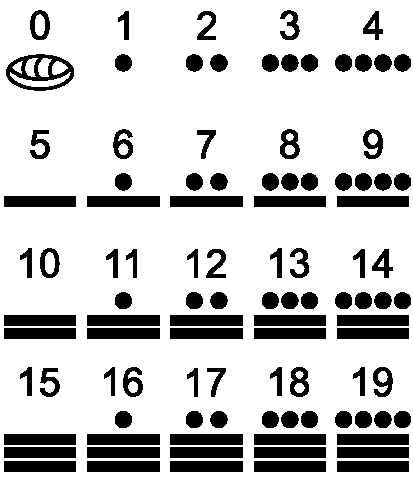
\includegraphics[width= 0.33 \textwidth]{maya.pdf}
        \caption{Exemplary image: Maya numerals.}
\label{fig:maya}
\end{figure}

If you download an image from Wikipedia or similar sources, please always check the applicable license terms. Most licenses require an adequate attribution. For Wikipedia, you can find the correct reference by clicking on the image and then clicking on the button saying 'use this file‘. Some licenses may have further restrictions, such as 'modifications are not allowed'. If modifications are allowed you may still have to mark those modifications. Please verify that you comply with all license requirements.

If you use your own images, please check if you still have the rights of use. The images may be copyrighted by your institution or a publisher of your previous publications.

%%% Wether a \clearpage before the image credits or the bibliography is a good idea, depends on the circumstances:
\clearpage

%%% Image credits: If you download an image form Wikipedia or similar sources, please always check the applicable license terms. Most licenses require an adequate attribution. For Wikipedia, you can find the correct reference by clicking on the image and then clicking on the button saying 'More details' and then on the link 'use this file' or similar. Some licenses may have further restrictions, such as 'modifications are not allowed'. If modifications are allowed you may still have to mark those modifications. Please verify that you comply with all license requirements. If you use your own images, please check if you still have the rights of use. The images may be copyrighted by your institution or a publisher of your previous publications.
\begin{imagecredits}
  \item[\autoref{fig:sample-image}] Archives of the Mathematisches Forschungsinstitut Oberwolfach,\\\url{https://www.mfo.de}, 2004.
  \item[\autoref{fig:maya}] ``Maya''. Author: Bryan Derkson. Licensed under Creative Commons Attribution-Share Alike 3.0 via Wikimedia Commons, \url{https://commons.wikimedia.org/wiki/File:Maya.svg}, visited on \printdate{2014-09-05}.
\end{imagecredits}

%%%%%%%%%%%%%%%% BIBLIOGRAPHY REVISITED %%%%%%%%%%%%%%%%%%%%%%%%%%%%%%%%%%%%%%%%%%%%%%%%%%%%%%%%%%%%%%%%%%
%%% 1. If you chose to use the embedded .bib file to provide your bibliographical references,
%%% leave the following command unchanged:
\bibliography{\jobname}
%%%
%%% 2. If you chose to use a separate .bib file, make the above command point to it,
%%% e.g. \bibliography{yourbibfile}. Give the file name without the extension .bib.
%%% Please do not forget to *submit* your .bib file together with your .tex file and
%%% your graphics files, if applicable.
%%% 
%%% 3. If you chose to use no BibTeX at all, delete the above \bibliography command
%%% and adopt the following lines as appropriate:
%%%
%\begin{thebibliography}{}
%\bibitem[1]{sample14}A. Candidate, {\slshape Thesis title}, PhD thesis, MFO, 2014.
%\bibitem[2]{sample11}C. Example, {\slshape A new perspective on mathematics}, New perspectives on arts and sciences, 2011.
%\bibitem[3]{knuth1984texbook}D. E. Knuth, {\slshape The TeXbook}, 1st ed., Addison-Wesley, 1984.
%\bibitem[4]{sample12}J.\ Sample, {\slshape Things you don't know about mathematics}, A bookseries about mathematics, Some publisher, 2012.
%\bibitem[5]{sample13}\underline{\hphantom{J.\ Sam}}\,, {\slshape Interesting facts in mathematics}, arxiv:8765.4321v1, 2013.
%\bibitem[6]{wikiMath}Wikipedia, {\slshape Mathematics --- {W}ikipedia{,} The Free Encyclopedia}, 2014, https://en.wikipedia.org/wiki/Mathematics, visited on May 19, 2014.
%\end{thebibliography}

\end{document}
